\documentclass{beamer}


\graphicspath{ {images/} }

\usetheme{Boadilla}

\title{Spotting Distracted Drivers}
\subtitle{HLCV Project}
\author[Reyes, Schaefer, Tonsen, Weber]{Guillermo Reyes \\
	 Daniel Schaefer \\
	 Marc Tonsen \\
 Dominik Weber\\}
 \institute[]{Saarland University}
\date{20.06.2016}



\begin{document}
	\begin{frame}
		\titlepage
	\end{frame}
	
	
	\begin{frame}
		\frametitle{Task}
		Kaggle CV Competition: State Farm Distracted Driver Detection \\
		Given a picture of the driver predict the probability of the following classes:
		
		\begin{columns}
			\begin{column}{0.5\textwidth}
				\begin{itemize}
					\item c0: safe driving
					\item c1: texting - right
					\item c2: talking on the phone - right
					\item c3: texting - left
					\item c4: talking on the phone - left
					\item c5: operating the radio
					\item c6: drinking
					\item c7: reaching behind
					\item c8: hair and makeup
					\item c9: talking to passenger			
				\end{itemize}
			\end{column}
			\begin{column}{0.5\textwidth}  %%<--- here
				\begin{center}
					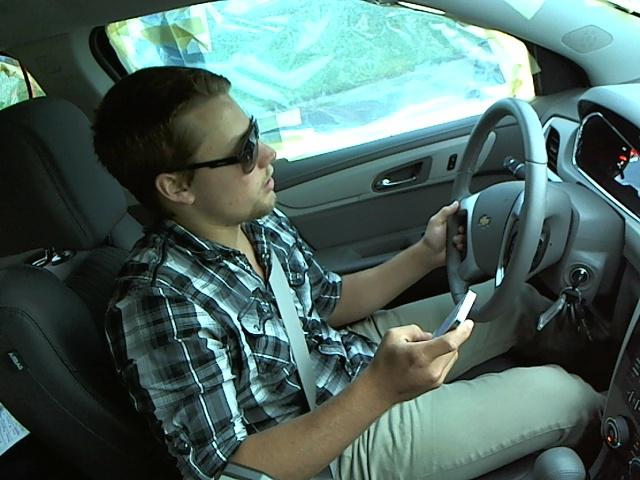
\includegraphics[width=0.9\textwidth]{img_6}
				\end{center}
			\end{column}
		\end{columns}
		
	\end{frame}
	
	
	\section{Tested but not working}	
    using all kinds of cascadeClassifier available in openCV. The results have been unsatisfactory so far mainly because our camera/face angle is very different, and even the profile detections don't work very well on pictures which come fairly close to being a profile view.  
    different haar-cascades for example face-boxer
    
    \begin{frame}
    	\frametitle{Classification based on the steering wheel}
    	Given the position of the hands on the steering wheel, several classes can be distinguished
    	\begin{columns}
    		\begin{column}{0.5\textwidth}
    			\centering
				c5 within the same car:
    			\begin{tabular}{c|cc}
    				& precision & recall \\ 
    				\hline rest & 0.86 & 0.97 \\ 
		    		c5 & 0.97 & 0.86 \\ 
    				\hline avg & 0.92 & 0.91 \\  
    			\end{tabular} 
    			
    			\vspace{0.5cm}
    			c5 whole dataset:
    			\begin{tabular}{c|cc}
    				& precision & recall \\ 
    				\hline rest & 0.68 & 0.76 \\ 
    				c5 & 0.71 & 0.62 \\ 
    				\hline avg & 0.70 & 0.69 \\  
    			\end{tabular} 
    		\end{column}
    		\begin{column}{0.5\textwidth}  %%<--- here
    			\begin{center}
    				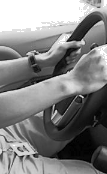
\includegraphics[width=0.3\textwidth]{steering_wheel1} \hspace{0.1cm}
    				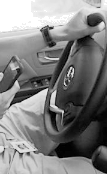
\includegraphics[width=0.3\textwidth]{steering_wheel2} \\\vspace{0.1cm}
    				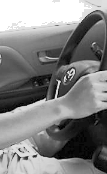
\includegraphics[width=0.3\textwidth]{steering_wheel3}\hspace{0.1cm}
    				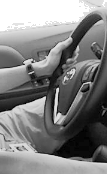
\includegraphics[width=0.3\textwidth]{steering_wheel4}
    				
    			\end{center}
    		\end{column}
    	\end{columns}
    	
    \end{frame}
    
     \begin{frame}
     	\frametitle{Classification based on the steering wheel}
     	Given the position of the hands on the steering wheel, several classes can be distinguished
     	\begin{columns}
     		\begin{column}{0.5\textwidth}
     			\begin{itemize}
     				\item Unbalanced data
     				\item Using weights does not help
     				\item[$\Rightarrow$] Artificially balance data
     				\vspace{0.3cm}
     				\item Raw Image as a feature
     				\item[$\Rightarrow$] Try SIFT/HoG features
     			\end{itemize}
     		\end{column}
     		\begin{column}{0.5\textwidth}  %%<--- here
     			\begin{center}
     				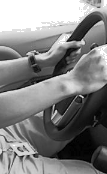
\includegraphics[width=0.3\textwidth]{steering_wheel1} \hspace{0.1cm}
     				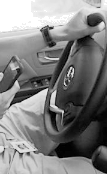
\includegraphics[width=0.3\textwidth]{steering_wheel2} \\\vspace{0.1cm}
     				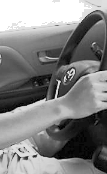
\includegraphics[width=0.3\textwidth]{steering_wheel3}\hspace{0.1cm}
     				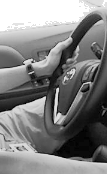
\includegraphics[width=0.3\textwidth]{steering_wheel4}
     				
     			\end{center}
     		\end{column}
     	\end{columns}
     	
     \end{frame}

	
	
\end{document}
